\documentclass{ctexbeamer}
\setbeamercolor{titlelike}{parent=structure,bg=lightgray}
\setbeamercovered{transparent}
\usefonttheme{structurebold}
\usetheme{CambridgeUS}
%\usecolortheme{rose}
%\usecolortheme{beaver}
\usecolortheme{crane}
\useoutertheme{infolines}

\usepackage{hyperref} 
\usepackage[backend=biber,style=authortitle]{biblatex}
%\usepackage[backend=bibtex,sorting=none]{biblatex}
%\addbibresource{main.bib}
%\setbeamerfont{footnote}{size=\tiny}

\renewcommand{\figurename}{Fig}


\title{MLIS2020: Some Security Issues on IoT Products with Home Network}

\author{Pan Lanlan (潘蓝兰) \newline  \newline abbypan@gmail.com} 
\institute[China]{Guangdong OPPO Mobile Telecommunications Corp. Ltd., China} 

\date{2020.09}

\begin{document}

\frame{\titlepage}

\frame{\tableofcontents}
\clearpage

\section{Offline Peer To Peer Connection}

\subsection{Bluetooth vs WiFi Direct}
\begin{frame}
\frametitle{Bluetooth vs WiFi Direct}

    https://www.dignited.com/23330/bluetooth-5-vs-wifi-direct-which-is-the-best-for-sharing-files-between-smartphones/

    \begin{figure}[H]
        \centering 
        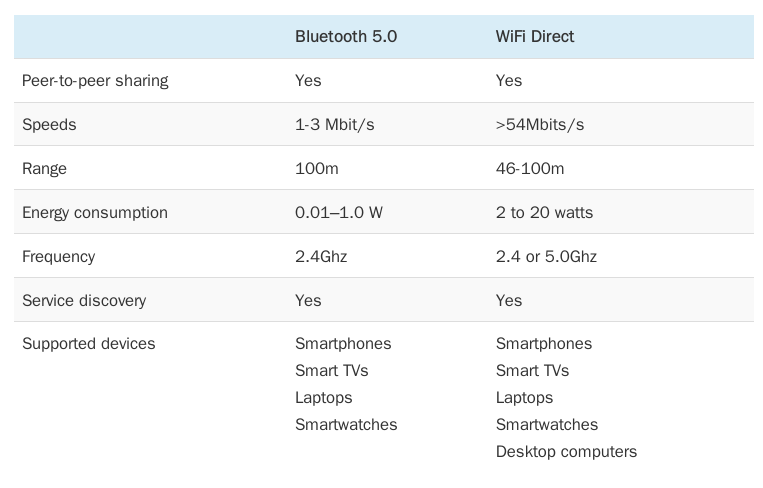
\includegraphics[width=0.7\textwidth]{pic/ble-wifi-direct.png} 
        \caption{Bluetooth vs WiFi Direct} 
        \label{fig.ble.wifi.direct}
    \end{figure}

\end{frame}

\subsection{Bluetooth}
\begin{frame}
\frametitle{Bluetooth Low Energy Pairing}

https://nvlpubs.nist.gov/nistpubs/SpecialPublications/NIST.SP.800-121r2.pdf

Pairing Methods: Numeric Comparison, Just Works, Passkey Entry, Out Of Band

    \begin{figure}[htbp]
        \centering
        \begin{minipage}[t]{0.48\textwidth}
            \centering
            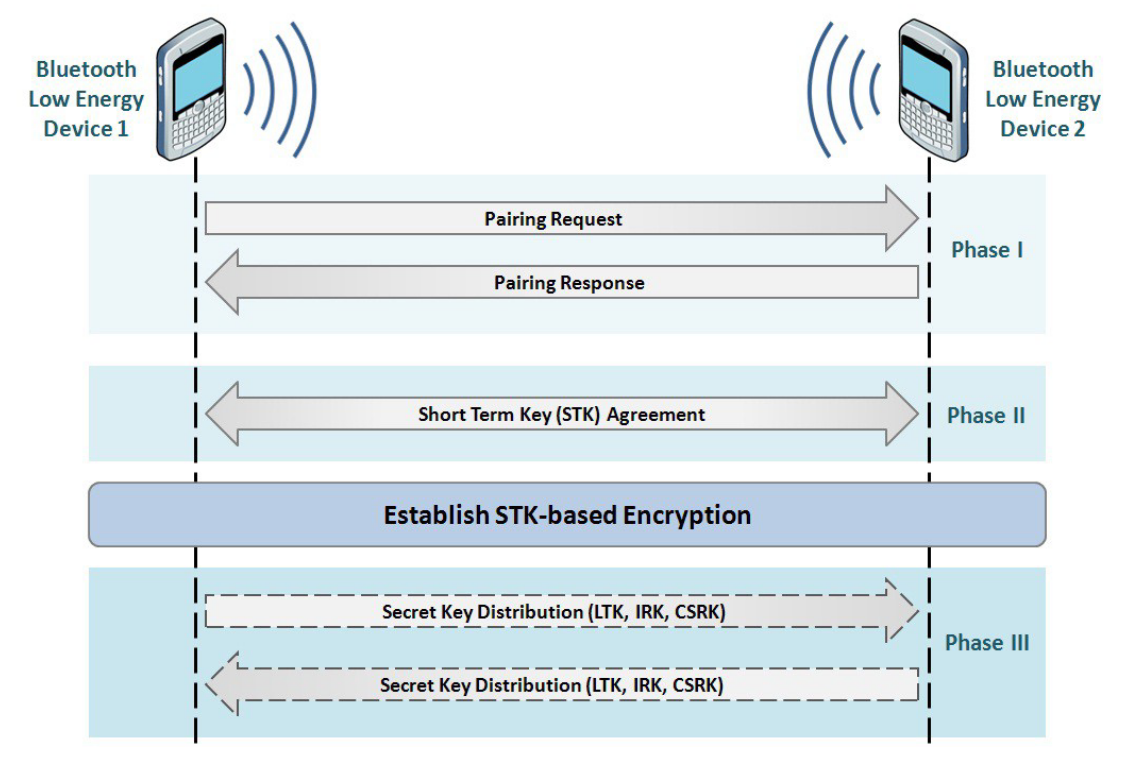
\includegraphics[width=0.9\textwidth]{pic/ble-legacy-pair.png}
            \caption{BLE Legacy Pairing}
        \end{minipage}
        \begin{minipage}[t]{0.48\textwidth}
            \centering
            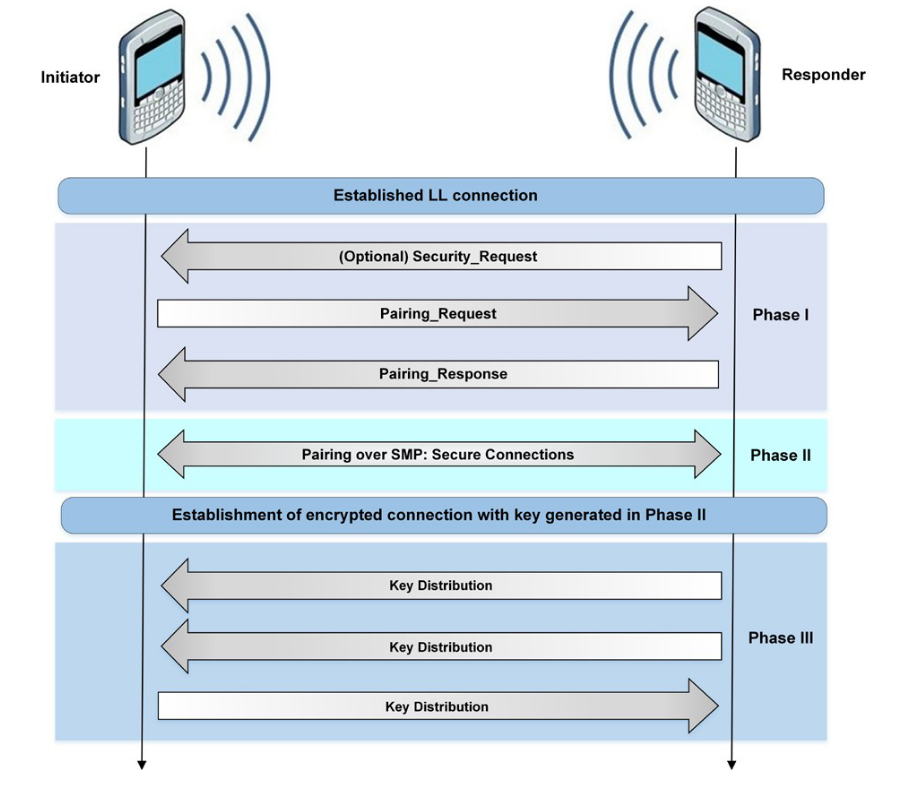
\includegraphics[width=0.9\textwidth]{pic/ble-secure-connect-pair.png}
            \caption{BLE Secure Connection Pairing}
        \end{minipage}
    \end{figure}

\end{frame}

\begin{frame}
\frametitle{Bluetooth Attack}

2019 \href{https://eprint.iacr.org/2019/1043.pdf}{Fixed Coordinate Invalid Curve Attack}: it is a MitM attack which modifies the public keys ina way that lets the attacker deduce the shared secret.
\newline
\newline
2019 \href{https://knobattack.com/}{KNOB (Key Negotiation of Bluetooth) Attack}: attacker forces two devices to use an 8-bit key, which can be brute-forced quite easily. 
\newline
\newline
    2020 \href{https://francozappa.github.io/about-bias/}{BIAS (Bluetooth Impersonation Attacks) Attack}: attacker completes secure connection establishment while impersonating Bluetooth master and slave devices, without having to know and authenticate the long term key shared between the victims.

\end{frame}

\subsection{Wifi Direct}
\begin{frame}
\frametitle{Wifi Direct Connection}

https://ieeexplore.ieee.org/document/7579020

    \begin{figure}[H]
        \centering 
        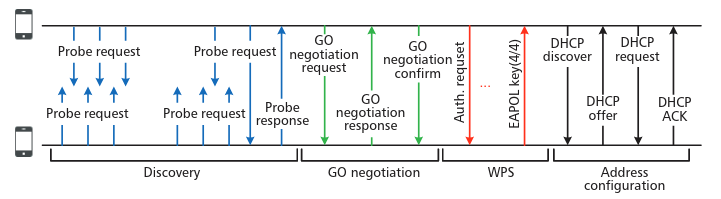
\includegraphics[width=0.8\textwidth]{pic/wifi-direct.png} 
        \caption{WiFi Direct Connection}
        \label{fig.wifi.direct}
    \end{figure}

\end{frame}

\begin{frame}
\frametitle{Wifi Attack}

    2017 \href{https://ieeexplore.ieee.org/document/8038416}{EvilDirect Attack}: a rogue GO accepts  the  clients  invitation  requests  beforethe  legitimate  GO,  to  hijack  the  wireless  communicationsbetween the clients and the legitimate GO.
\newline
\newline
    2017 \href{https://www.krackattacks.com/}{Key Reinstallation Attacks (KRACKs)}: an attacker can force nonce resets by collecting and replaying retransmissions of message 3 of the 4-way handshake. By forcing nonce reuse in this manner, the encryption protocol can be attacked, e.g., packets can be replayed, decrypted, and/or forged.
\newline
\newline
2019 \href{https://arstechnica.com/information-technology/2019/10/unpatched-linux-flaw-may-let-attackers-crash-or-compromise-nearby-devices/}{RTLWIFI driver vulnerability (CVE-2019-17666)}: The vulnerability triggers a buffer overflow in the Linux kernel when a machine with a Realtek Wi-Fi chip is within radio range of a malicious device. At a minimum, exploits would cause an operating-system crash and could possibly allow a hacker to gain complete control of the computer.
    

\end{frame}

\subsection{Application Level Authentication}
\begin{frame}
\frametitle{Application Level Authentication}

For home network scenario, IoT product should add application level authentication over Bluetooth/WiFi Direct.
\newline
\newline
generate random password on initial binding (such as scan QR code)
\newline
secure communication with balanced PAKE protocol.

    \begin{figure}[H]
        \centering 
        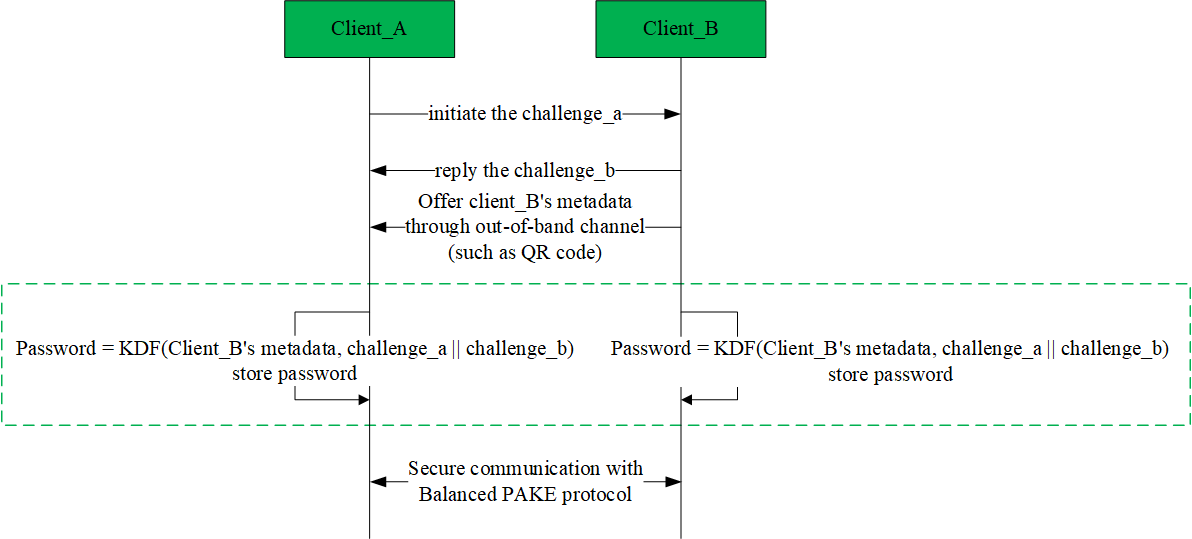
\includegraphics[width=0.75\textwidth]{pic/pake.png} 
        \caption{Application Level Authentication} 
        \label{fig.pake}
    \end{figure}

\end{frame}

\section{Communications Between Multiple IoT products}

\subsection{Binding}
\begin{frame}
\frametitle{Binding}

User controls the actuators (such as Air Condition, TV, Light) with commanders (such as Mobile Phone, Smart Speaker).

Router isn't involved in the communications, just forwards the packets. 

Different actuator products should be adapted to different commanders' platform.

    \begin{figure}[H]
        \centering 
        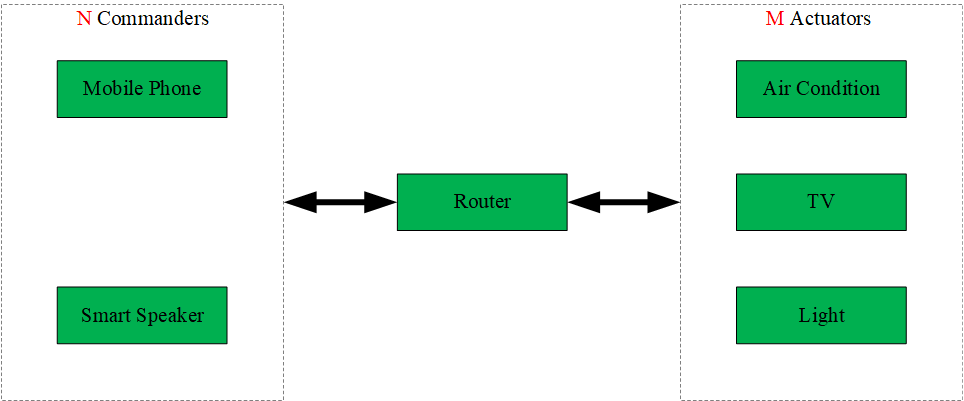
\includegraphics[width=0.8\textwidth]{pic/smart_home.png} 
        \caption{N Commanders and M Actuators: (N x M) initiate binding} 
        \label{fig.smart.home}
    \end{figure}

\end{frame}

\subsection{Router Centered ECQV Implicit Certificate System}
\begin{frame}
\frametitle{Router Centered ECQV Implicit Certificate System}

User controls the actuators (such as Air Condition, TV, Light) with commanders (such as Mobile Phone, Smart Speaker).

Router acts as the center credential distributor of the home network.

Both N Commanders and M Actuators request ECQV Implicit Certificate from Router for initiate binding.

    \begin{figure}[H]
        \centering 
        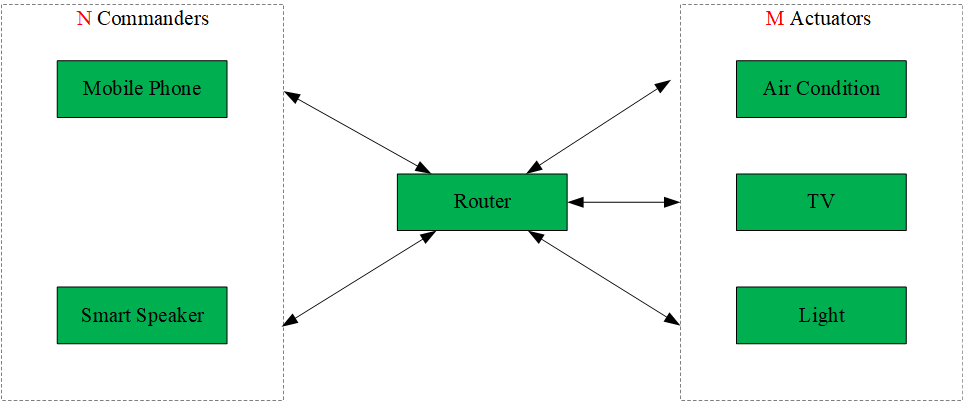
\includegraphics[width=0.8\textwidth]{pic/ecqv.png} 
        \caption{N Commanders and M Actuators: (N + M) initiate binding} 
        \label{fig.ecqv}
    \end{figure}

\end{frame}

\subsection{ECQV Implicit Certificate Provision}
\begin{frame}
\frametitle{ECQV Implicit Certificate Provision}

https://www.secg.org/sec4-1.0.pdf

    U:  IoT Products

    CA: Router

    \begin{figure}[H]
        \centering 
        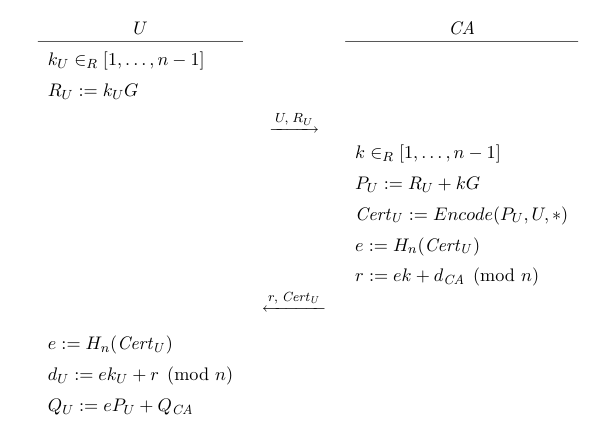
\includegraphics[width=0.6\textwidth]{pic/ecqv_provision.png} 
        \caption{Router Generate ECQV Implicit Certificate For IoT Products} 
        \label{fig.ecqv.provision}
    \end{figure}

\end{frame}

\section{Local Visit To Home Gateway Service}

\subsection{Router Web Admin Page}
\begin{frame}
\frametitle{Router Web Admin Page}

Home Gateway (Router) doesn't deploy X.509v3 Certificate which is issued by public CA.

To avoid the browser's invalid certificate alarm, router's web service has to accept local client's visit without TLS connection.

Even worse, some router may set the Web Admin Password same as Wi-Fi Password.

    \begin{figure}[H]
        \centering 
        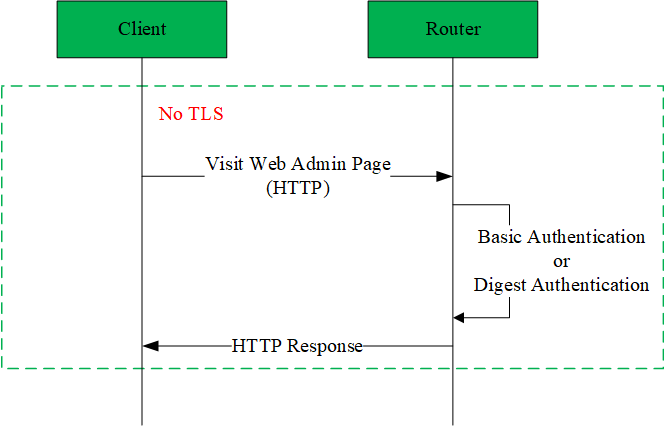
\includegraphics[width=0.5\textwidth]{pic/web_adm.png} 
        \caption{Local Visit to Router Web Admin Page Without TLS} 
        \label{fig.web.adm}
    \end{figure}

\end{frame}

\subsection{Router DNS Service}
\begin{frame}
\frametitle{Router DNS Service}

Router offer DNS forward resolver service for local clients.

Default router's DNS service is in plaintext.

    \begin{figure}[H]
        \centering 
        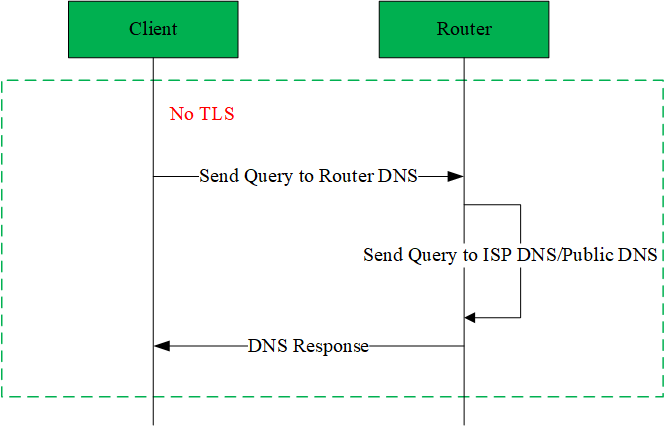
\includegraphics[width=0.5\textwidth]{pic/router_dns.png} 
        \caption{Local Visit to Router DNS Service Without TLS} 
        \label{fig.router.dns}
    \end{figure}

\end{frame}

\subsection{Use TLS-PSK}
\begin{frame}
\frametitle{Use TLS-PSK}

Router can reuse Wi-Fi password or setup specific password for TLS :  
    \begin{itemize}
\item        tls-psk = kdf(Wi-Fi User Name, Wi-Fi User Password) 

    \item    tls-psk = kdf(Wi-Fi Password)

       \item  tls-psk = kdf(TLS Specific Password)
    \end{itemize}

Client can make secure connection with Router if its system support TLS-PSK.

    \begin{figure}[H]
        \centering 
        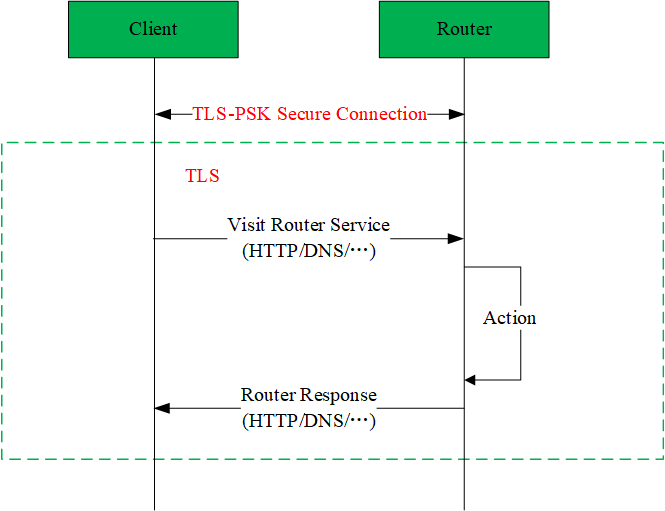
\includegraphics[width=0.4\textwidth]{pic/tls_psk.png} 
        \caption{Local Visit to Router Service With TLS-PSK} 
        \label{fig.tls.psk}
    \end{figure}

\end{frame}

\section{Conclusion}

\subsection{Conclusion}
\begin{frame}
\frametitle{Conclusion}

Smart home network should be based on a platform that can secure control smart IoT products.
\newline
\newline
We should build up the open IoT ecosystem with secure design.
\newline
\newline

\end{frame}

%\subsection{Resources}
%\begin{frame}{Resources}

    %\begin{thebibliography}{99}
        %\bibitem{rtlwifi} RTLWIFI
            %https://arstechnica.com/information-technology/2019/10/unpatched-linux-flaw-may-let-attackers-crash-or-compromise-nearby-devices/
    %\end{thebibliography}

%\end{frame}


\end{document}
